\documentclass{article}
\usepackage{graphicx} % Required for inserting images

\title{Notes}
\author{Cate Dunham}
\date{August 2024}

\begin{document}

\maketitle

\section{Thoughts for Model Development}

Using FCD (Frechete ChemNet Distance) instead of/in addition to MSE for encoder's loss. FCD is based on chemistry principles. 
One of the torch FCD functions is a distance measurement, use that.

\section{Dynamical Systems}

% \section{Questions:}
% Why do we differentiate between discrete and continuous time? In the example in \textit{Invitation to Dynamical Systems}, 
% it seemed as though if you were to ``zoom out'', discrete time is really just continuous (why does it matter if the space between )

\subsection{Vocabulary:}
\begin{itemize}
    \item Derivative - rate of change
    \item State - variable $x$
    \item Time course - trajectory of $x$ (how $x$ changes over time $t$)
    \item Rate of change (slope) $\frac{dx}{dk}$ - $\dot{x}$
\end{itemize}

\subsection{Overview:}
In a dynamical system the state $x$ changes over time $t$.

We aim to find a function $f$ that describes how $x$ changes over $t$, 
\begin{equation}
    f(x(t)).
\end{equation}

Once we have $f$ we can compute all values of $x$ as shown in Figure \ref{fig:dynamical_systems_iteration}.
\begin{figure}[H]
    \centering
    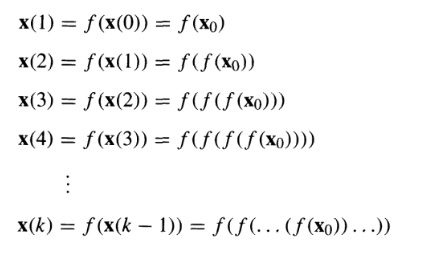
\includegraphics[width=90mm]{images/dynamical_systems_iteration.png}
    \caption{Iterating $f(x)$ to find the value of $x$ at time $t$. Note that time above is denoted as $k$ as the image was describing a discrete time system.}
    \label{fig:dynamical_systems_iteration}
\end{figure}


% General form of discrete dynamical system:
% \begin{equation}
%     f(x(t)).
% \end{equation}

\subsection{Topics for further learning:}
Differential equations.

\subsection{Resources:}
Helpful indtroduction to dynamical systems: https://www.youtube.com/watch?v=A6R183ZIxC8
Invitation to dynamical systems by ER Scheinerman
Berkeley research on dynamical systems and machine learning: https://www.stat.berkeley.edu/~mmahoney/talks/dynamical_systems_and_ml_2.pdf

\end{document}